\documentclass[12pt,a4paper]{ThesisClass}
\usepackage{pdfpages}
\usepackage[utf8]{inputenc}
\usepackage[english]{babel}
\usepackage{amsmath}
\usepackage{amsfonts}
\usepackage{amssymb}
\usepackage{graphicx}
\usepackage[citestyle=authoryear,giveninits=true,style=bwl-FU,natbib=true,backend=bibtex,maxnames=3]{biblatex}
\AtEveryBibitem{%
  \clearlist{language}%
}
\usepackage{url}         
\usepackage{algorithm}
\usepackage[noend]{algpseudocode}
\usepackage[toc,page]{appendix}
\usepackage{enumitem}
\usepackage{hyperref}
\usepackage{url}
\usepackage{hyperref}
\usepackage{geometry}
\usepackage{color}
\usepackage{lscape}
\usepackage{float}
\usepackage{longtable}
\usepackage{supertabular}
\usepackage[export]{adjustbox}
\usepackage{csquotes}
\usepackage{listings}
\usepackage{color}
\usepackage{tocloft}

\setlength\cftaftertoctitleskip{0pt}

\definecolor{codegreen}{rgb}{0,0.6,0}
\definecolor{codegray}{rgb}{0.5,0.5,0.5}
\definecolor{codepurple}{rgb}{0.58,0,0.82}
\definecolor{backcolour}{rgb}{0.95,0.95,0.92}
\lstdefinestyle{mystyle}{
    backgroundcolor=\color{backcolour},   
    commentstyle=\color{codegreen},
    keywordstyle=\color{magenta},
    numberstyle=\tiny\color{codegray},
    stringstyle=\color{codepurple},
    basicstyle=\footnotesize,
    breakatwhitespace=false,         
    breaklines=true,                 
    captionpos=b,                    
    keepspaces=true,                 
    %numbers=left,                    
    %numbersep=5pt,                  
    showspaces=false,                
    showstringspaces=false,
    showtabs=false,                  
    tabsize=2
}
\lstset{style=mystyle}

\linespread{1.5}
\setlength{\headsep}{1.0cm} %separador entre header e body
\newcommand*\rfrac[2]{{}^{#1}\!/_{#2}} %sided fraction
\makeatletter
\setlength{\@fptop}{0pt}
\makeatother


\bibliography{bibliography.bib}
\setcounter{secnumdepth}{3}
\setcounter{tocdepth}{3}

%----------------------------------------------------------------------------------
%	O documento começa aqui
%----------------------------------------------------------------------------------
\begin{document}

\includepdf[fitpaper, page=1]{Capa1.pdf}
\thispagestyle{empty}
\cleardoublepage

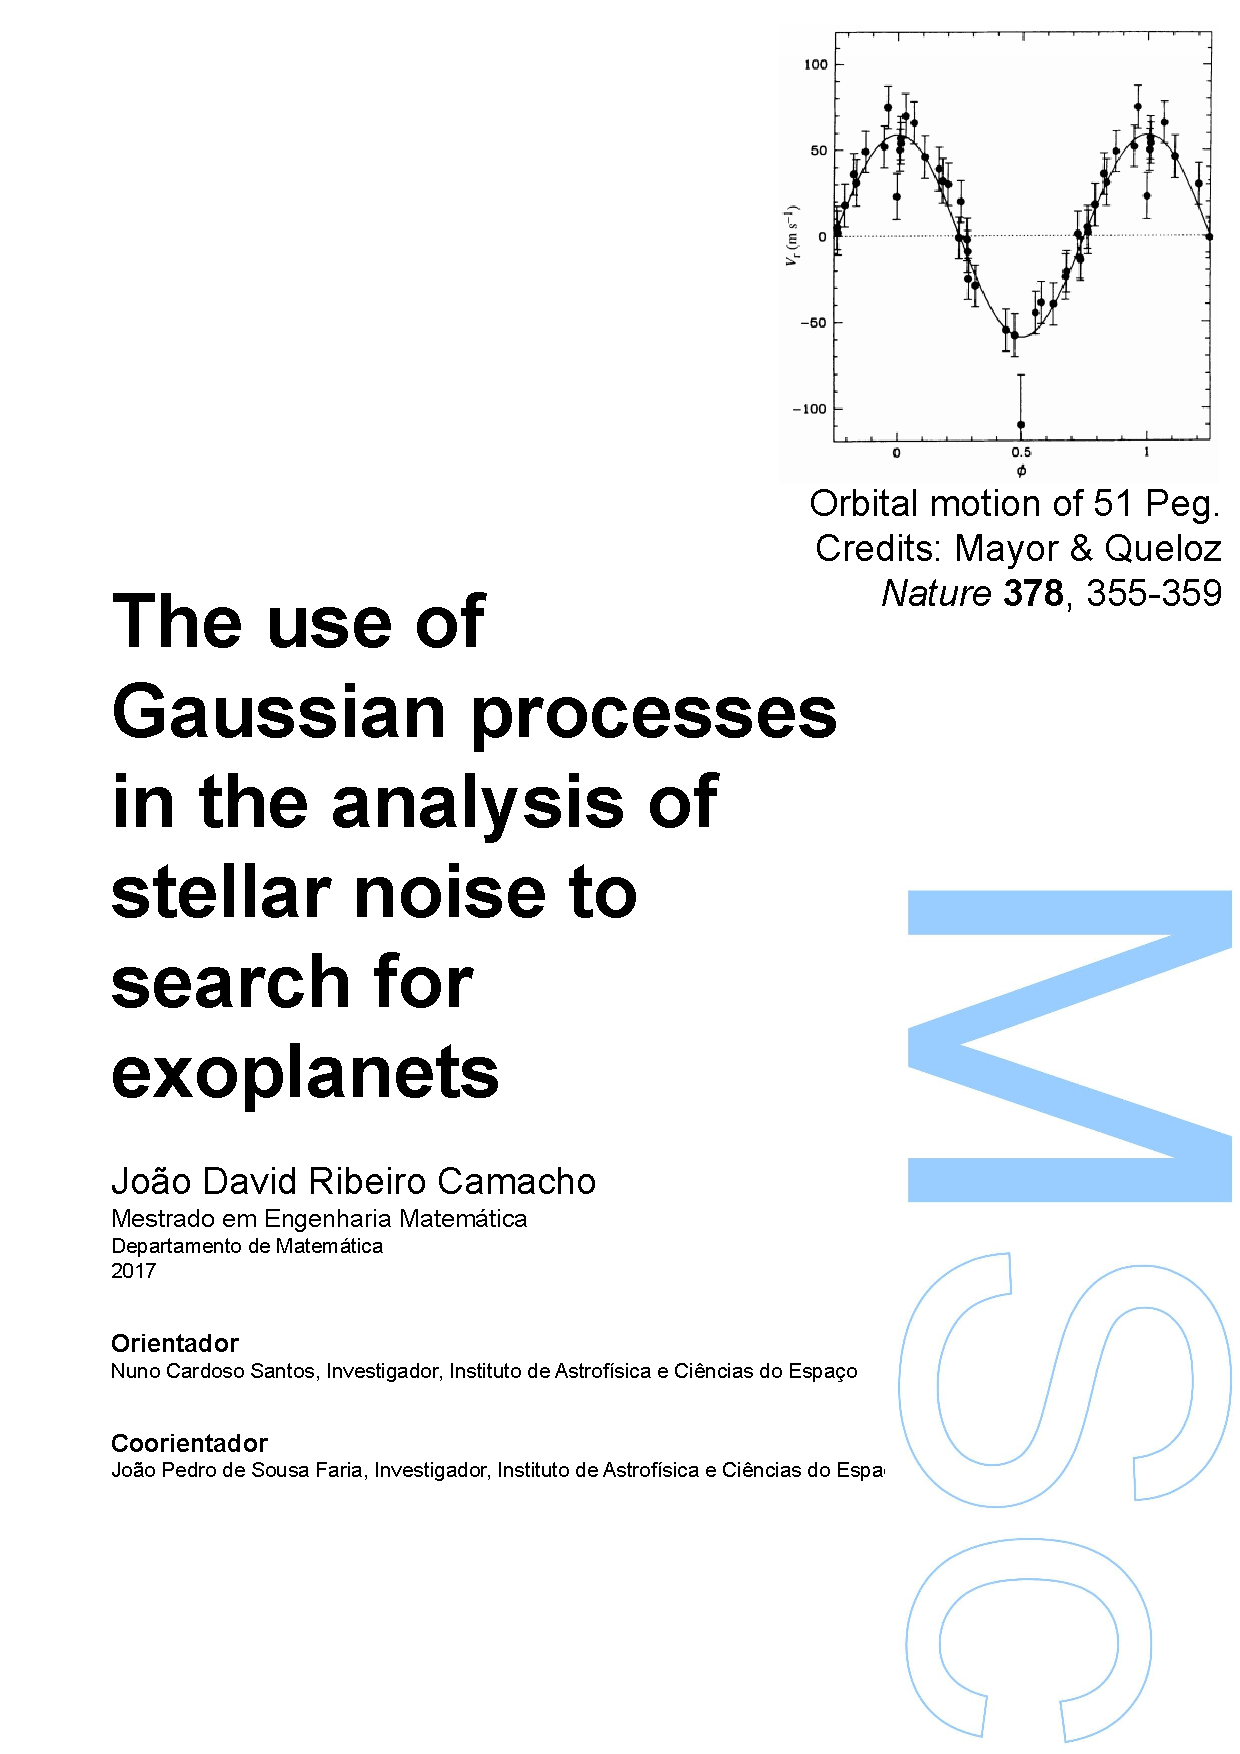
\includepdf[width=\paperwidth, page=1]{Capa2.pdf}
\thispagestyle{empty}
\newpage
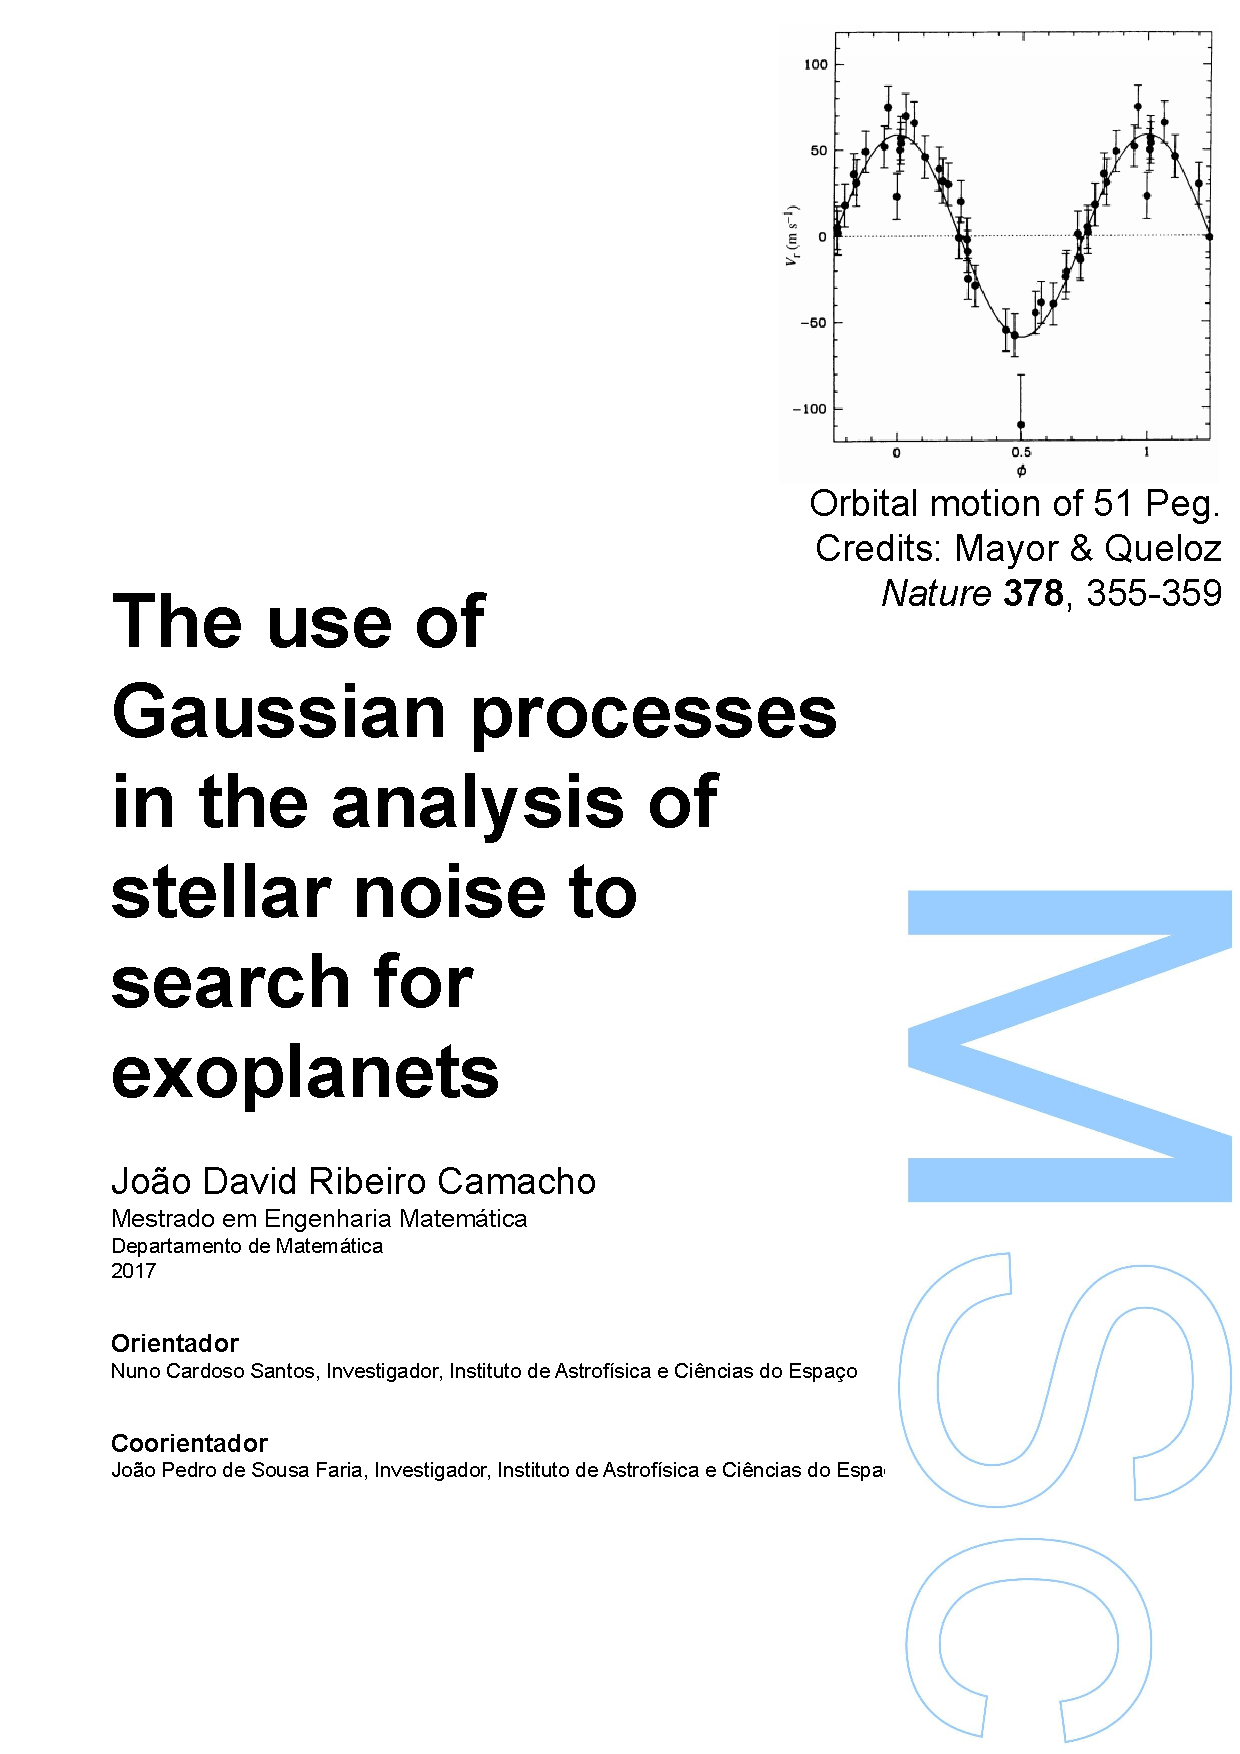
\includepdf[width=\paperwidth, page=2]{Capa2.pdf}
\thispagestyle{empty}
\newpage


\university{Faculdade de Ciências da Universidade do Porto}
\title{Titulo da tese}
\degree{Master in Mathematical Engineering Dissertation}
\author[1,2]{O vosso nome}
\supervisor[1,2]{O nome do supervisor}
\affil[1]{Afiliações tipo departamentos e centros de investigação}
\affil[2]{Afiliações tipo departamentos e centros de investigação}
\date{}

\pagenumbering{roman} % Start roman numbering
%----------------------------------------------------------------------------------
%	Resumo
%----------------------------------------------------------------------------------
\chapter*{Resumo}

%----------------------------------------------------------------------------------
%	Abstract
%----------------------------------------------------------------------------------
\chapter*{Abstract}

%----------------------------------------------------------------------------------
%	Acknowledgements
%----------------------------------------------------------------------------------
\chapter*{Acknowledgements}


\cleardoublepage
\newpage
\tableofcontents
\newpage
\listoffigures
\newpage
\listoftables 


%----------------------------------------------------------------------------------------
%	Introduction
%----------------------------------------------------------------------------------------
\FloatBarrier
\newpage
\pagenumbering{arabic} % Switch to normal numbers
\chapter{Introduction}\label{ch:00intro}
\begin{center}
\begin{minipage}{15cm}
\textit{"Frase inspiradora se gostarem dessas cenas, caso contrário apaguem."}

\hfill João Camacho (1990-)\\
\end{minipage}
\end{center}


%----------------------------------------------------------------------------------------
%	Chapter 1
%----------------------------------------------------------------------------------------
\FloatBarrier
\newpage
\chapter{Titulo do 1o capitulo}\label{ch:01cap1}
\begin{center}
\begin{minipage}{15cm}
\textit{"Frase inspiradora se gostarem dessas cenas, caso contrário apaguem."}

\hfill João Camacho (1990-)\\
\end{minipage}
\end{center}

\section{secção}

\subsection{subsecção}


%----------------------------------------------------------------------------------------
%	Chapter 2
%----------------------------------------------------------------------------------------
\FloatBarrier
\newpage
\chapter{Titulo do 2o capitulo}\label{ch:02cap2}
\begin{center}
\begin{minipage}{15cm}
\textit{"Frase inspiradora se gostarem dessas cenas, caso contrário apaguem."}

\hfill João Camacho (1990-)\\
\end{minipage}
\end{center}

\section{secção}

\subsection{subsecção}


%----------------------------------------------------------------------------------
%	Bibliography
%----------------------------------------------------------------------------------
\FloatBarrier
\newpage
\printbibliography


%----------------------------------------------------------------------------------
%	Apendices
%----------------------------------------------------------------------------------
\FloatBarrier
\newpage
\begin{appendices}
\chapter{1o apendice}\label{apx:01apendix}


\end{appendices}
\end{document}